\section{Part a}
Michaelis-Menten enzymes follow simple first order kinetics, i.e. the rate of the reaction depends only on  one of the reactants, the substrate. If we let $S_{1}$ be the substrate, $S_{2}$ be the enzyme, $S_{3}$ be the enzyme-substrate complex and $S_{4}$ be the resultant product, then we can write a chemical reaction for the transformation of $S_{1}$ in  $S_{4}$ as\\

$S_{1}$ + $S_{2}$  $\xrightarrow{\mbox{\tiny{$c_{1}$}}} S_{3}$\\


$S_{3}$ $\xrightarrow{\mbox{\tiny{$c_{2}$}}} S_{1} + S_{2}$\\


$S_{3}$ $\xrightarrow{\mbox{\tiny{$c_{3}$}}} S_{2} + S_{4}$,\\

where $c_{1}$, $c_{2}$, $c_{3}$ are the rate constants for each reaction.\\
Let a cell of \textit{E.Coli} have $S_{1}$=500 molecules of substrate, $S_{2}$=50 molecules of enzyme and $S_{3}=S_{4}=0$, when the reaction begins. The rate constants satisfy:
$$
c_{1} = 0.002, c_{2} = 6 \cdot 10^{-5}, c_{3} = 0.08.
$$
We develop a Gillespie Algorithm for these Michaelis-Menten enzyme reactions and present 2 distinct simulations of the time series for $t \in [0,200]$, using the same rate constants listed above. Below is the code built \newpage
\begin{lstlisting}[style=A]
% LV_gill.M
% Simple implementation of the Stochastic Simulation Algorithm
% (or Gillespie's algorithm) for the Lotka-Volterra system.
%
% rand('state',100) % Can fix rand # pattern
% stoichiometric matrix for rxs
V = [-1 1 0;-1 1 1;1 -1 -1;0 0 1];
%%%%%%% Parameters and Initial Conditions
X = zeros(4,1);
X(1) = 500;   % initial molecules of S1 (substrate)
X(2) = 50;   % initial molecules of S2 (enzyme)
X(3) = 0;   % initial molecules of S3 (enzyme-substrate complex)
X(4) = 0;   % initial molecule of S4 (product)

Y1(1) = X(1);  % store # of molecules
Y2(1) = X(2);
Y3(1) = X(3);
Y4(1) = X(4);

% set chem rx coefficients
c(1) = 0.002; c(2) = 0.00006; c(3) = 0.08;
t = 0;         % initial time
T(1) = t;
tfinal = 200;   % final time
i = 1;
while t < tfinal
% rx combination functions
a(1) = c(1)*X(1)*X(2);
a(2) = c(2)*X(3);
a(3) = c(3)*X(3);
asum = sum(a);  % total a
% generate rand # and find rx occurring
j = min(find(rand<cumsum(a/asum)));
% 2nd rand # for time until rx
tau = log(1/rand)/asum;
X = X + V(:,j); % Stochastic matrix adjusts X
t = t + tau;
i = i + 1;
T(i) = t;
Y1(i) = X(1);
Y2(i) = X(2);
Y3(i) = X(3);
Y4(i) = X(4);
figure(101)
plot(T,Y1,'b-',T,Y2,'r-',T,Y3,'m-',T,Y4,'g-');grid;
xlim([0,200]);
fontlabs = 'Times New Roman'; % Font type used in labels
xlabel('$t$','FontSize',14,'FontName',fontlabs,...
'interpreter','latex');  
ylabel('Molecules','FontSize',14,'FontName',fontlabs);  
set(gca,'FontSize',12);
legend('S1','S2','S3','S4','location','best');
title('Michaelis-Menten Enzyme Reactions using Gillespie Algorithm');
\end{lstlisting}


The following figure shows two different simulations of the time series $t \in [0,200]$ for all 4 chemical species

\begin{figure}[H]
	\subfigure[]{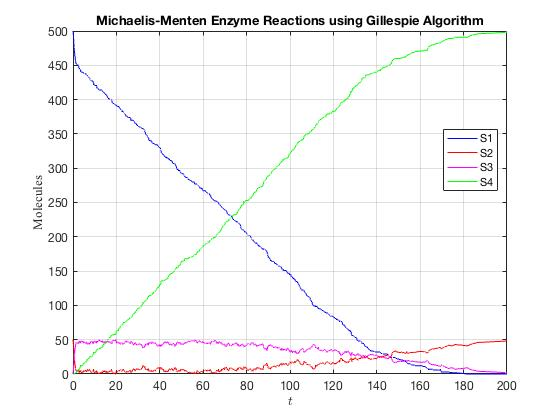
\includegraphics[scale=0.75]{Gillespie_Prob5a1.jpg}}
	\subfigure[]{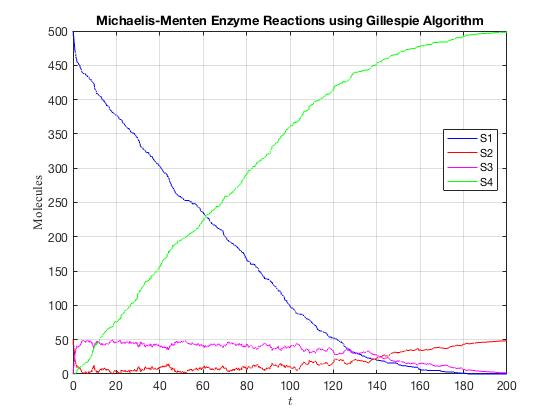
\includegraphics[scale=0.75]{Gillespie_Prob5a2.jpg}}
	\caption{a)First Simulation; b) Second Simulation}
\end{figure}

In Figure 5.1a we see that the concentration of the substrate $S_{1}$ (blue line) steadily decreases as time goes on, resembling an exponential decay, from its initial value of 500 molecules at $t=0$ to asymptotically approaching zero. The almost exact opposite "route" is followed by the product $S_{4}$,(green line) whose concentration that starts obviously at zero molecules and steadily increases, levelling off at around 500 molecules. The concentrations of the two chemical species crosses each other at around $t=70$.\\
As for the enzyme concentration $S_{2}$ (red line), it start at 50 molecules, almost instantaneously drops close to zero and seems to oscillate between zero and 10 molecules up until $t=80$, when it appears to more steadily increases all the way until $t=200$ when it comes back to 50 molecules. This is in accord with enzyme kinetics, as the enzyme regenerates after the formation of the product, getting ready to catalyse a new reaction. The enzyme-substrate complex follows almost exactly the opposite "route" of the enzyme, and we can see that its concentration $S_{3}$ (magenta line) starts at zero and almost immediately peaks at around 50 molecules, where it stays pretty much constant, with some minor fluctuations, up until $t=80$ when it seems to be more steadily decreasing up until $t=200$ when it reaches zero. The enzyme concentration and the enzyme-substrate complex concentration cross their paths at around $t=143$, and they cross the substrate concentration almost immediately after, the enzyme at $t=145$, while the enzyme-substrate complex at $t=150$ .\\
All of this is in accordance with what we know about enzyme kinetics, as the enzyme is regenerated at the end of the reaction and with the law of concentration of mass, as we start with a total of 550 molecules and we end up with a total of 550 and 50 molecules.\\

In Figure 5.1b we see that the concentration of the substrate $S_{1}$ (blue line) steadily decreases as time goes on, resembling an exponential decay, from its initial value of 500 molecules at $t=0$ to asymptotically approaching zero. The almost exact opposite "route" is followed by the product $S_{4}$,(green line) whose concentration that starts at zero molecules and then steadily increases to level off at around 500 molecules. The concentrations of the two chemical species cross each other at around $t=61$.\\
As for the enzyme concentration $S_{2}$ (red line), it start at 50 molecules, and drops close to zero at around $t=5$, then seems to oscillate between zero and 10 molecules up until $t=80$, when it appears to more steadily increases all the way until $t=200$ when it comes back to 50 molecules. This is in accord with enzyme kinetics, as the enzyme regenerates after the formation of the product, getting ready to catalyse a new reaction. The enzyme-substrate complex follows almost exactly the opposite "route" of the enzyme, and we can see that its concentration $S_{3}$ (magenta line) starts at zero and peaks at around 50 molecules at around $t=5$, then it stays pretty much constant, with some minor fluctuations, up until $t=80$ when it seems to be more steadily decreasing up until $t=200$ when it reaches zero. The enzyme concentration and the enzyme-substrate complex concentration cross their paths at around $t=143$, after having crossed the path of the concentration of the substrate, the enzyme at $t=139$, while the enzyme-substrate complex at $t=130$ respectively.\\
All of this is in accordance with what we know about enzyme kinetics, as the enzyme is regenerated at the end of the reaction and with the law of concentration of mass, as we start with a total of 550 molecules and we end up with a total of 550 and 50 molecules.\\
\section{Part b}
We can rewrite the reactions of Part a) as system of 4 differential equations, as follows
$$
\frac{d[S_{1}]}{dt} = -c_{1}[S_{1}][S_{2}] + c_{2}[S_{3}]
$$
$$
\frac{d[S_{2}]}{dt} = -c_{1}[S_{1}][S_{2}] + (c_{2}+c_{3})[S_{3}]
$$
$$
\frac{d[S_{3}]}{dt} = c_{1}[S_{1}][S_{2}] - (c_{2}+c_{3})[S_{3}]
$$
$$
\frac{d[S_{4}]}{dt}  = c_{3}[S_{3}],
$$
where $[S_{1}]$, $[S_{2}]$, $[S_{3}]$, $[S_{4}]$ are the concentration of the substrate, the enzyme, the enzyme-substrate complex and the product respectively.\\
The figure below shows a graph of the ODE simulation (Figure 5.2a) by itself and a graph of the ODE simulation overlayed with one from the Gillespie stochastic simulation algorithm for the same reactions.

\begin{figure}[H]
	\subfigure[]{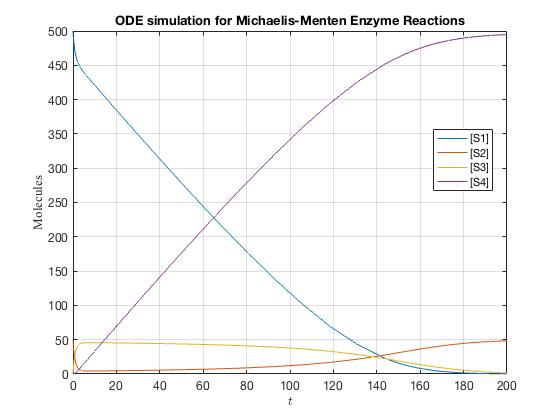
\includegraphics[scale=0.75]{Gillespie_Prob5b1.jpg}}
	\subfigure[]{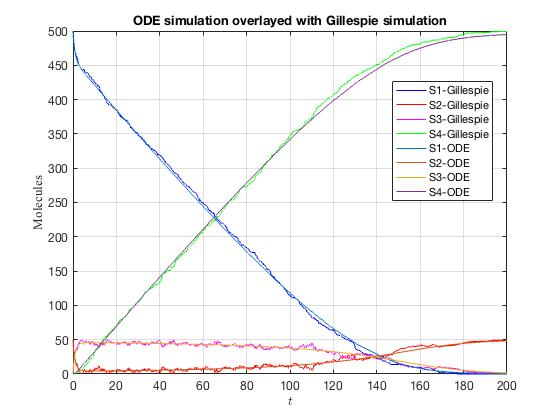
\includegraphics[scale=0.75]{Gillespie_Prob5b2.jpg}}
	\caption{a)ODE simulation; b) ODE vs. Gillespie Simulation}
\end{figure}

Figure 5.2 shows how the Gillespie Algorithm and the ODE simulation compare to each other. The overall trend appears to be basically the same, with the ODE simulation giving smoother graphs, whereas the Gillespie Algorithm has more "irregular" paths. Obviously the ODE simulation assume the reaction to be happening in a continuous manner, such that there are no corners or irregularities in the graphs, whereas the Gillespie Algorithm uses a stochastic approach and allows small fluctuations to happen among the concentrations of the different chemical species, giving, in this regard, a more realistic picture of the evolution of the reaction. In fact, it's unlikely that the concentration of the various species will just follow a smooth path from the beginning to the end of the reaction, as there are many factors that could alter the stability of the system at any given moment and the Gillespie Algorithm takes into account the different probabilities that the species interact with each other at any given moment.\\
That being said, both approaches give the same general trend for the overall reaction.

\section{Part c}
Using the quasi-steady state approximation, the Michaelis-Menten enzyme reactions can be re-written as the following system of differential equations
$$
\frac{ds_{1}}{dt} = - \frac{V_{m}s_{1}}{K_{m}+s_{1}}
$$
$$
\frac{ds_{4}}{dt} = \frac{V_{m}s_{1}}{K_{m}+s_{1}},
$$
where $s_{1}$ and $s_{4}$ are the concentration of the substrate and the product respectively, and $V_{m}$ and $K_{m}$ are kinetic constants.\\
So, our first estimate of the two parameters is done by applying some basic knowledge about Michaelis-Menten enzyme kinetics:
$$
V_{m} = c_{2}[S_{2}]_{t=0} \rightarrow  V_{m} = 4,
$$
$$
K_{m} = \frac{c_{2}+c_{3}}{c_{1}} \rightarrow K_{m} = 40.03,
$$
where $[S_{2}]$ is the concentration of the enzyme at the beginning of the reaction (i.e. 50 molecules in our case), and $c_{1}$, $c_{2}$, $c_{3}$ are the kinetic constants given in Part a.\\
So from here, we build a MatLab code to optimise $V_{m}$ and $K_{m}$ using fminsearch and we find the optimal values to be
$$
V_{m} = 4.8224,
$$
$$
K_{m} = 88.9313.
$$
The sum of square errors is found to be
$$
SSE =  12588
$$
Below is a graph for the simulations of the systems in Parts b and c 
\begin{figure}[H]
	\subfigure{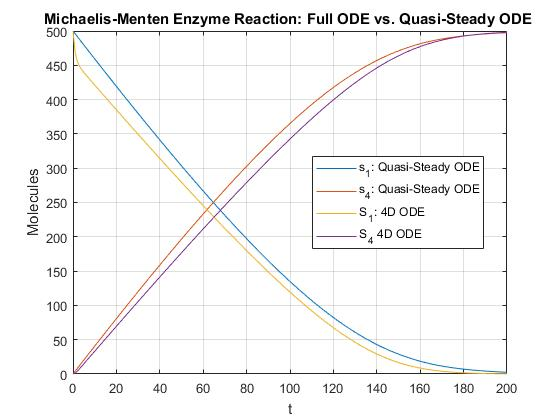
\includegraphics[scale=0.75]{Gillespie_Prob5c.jpg}}
	\caption{4D-ODE Simulation vs. Quasi-Steady State Simulation }
\end{figure}
Figure 5.3 shows that for both simulation the overall trend is the same, as the concentration on the product steadily decreases until it gets to zero (or very close to it), while the concentration of the product steadily increases until it gets to 500 (or very close to it), as expected.\\
However, a couple of differences can be noticed right away: first of all, according to the system build in Part b, the concentration of the product almost instantaneously drops from its starting value of 500 to 450 molecules, whereas in the quasi-steady state simulation the path of the substrate is smoother, with no abrupt drops. Interestingly, the substrate and the product cross each other at the same time in both simulation (around $t=70$), however, at that point in time, substrate and product have different concentrations in the two simulations: in the 4D-ODE simulation of Part b, when they intersect they both have around 225 molecules, whereas in the quasi-steady state simulation when they intersect they both have about 250 molecules, which corresponds to half the initial concentration of the substrate and half the final concentration of the product.\\
As for the product, both simulations have the same overall trend, but the quasi-steady state simulation shows a faster increase in its concentration if compared to the simulation run in Part b.

\section{Part d}
To convert from molecules to mole, we divide the number of molecules by the Avogadro number, which is given by
$$
N_{A} \approx 6.022 \cdot 10^{23} molecules/mole.
$$
We are given that the volume of the $\textit{E.Coli}$ is
$$
V = 7 \cdot 10^{-19}L
$$
Therefore the conversion from $\textit{molecules/E.Coli}$ to $\textit{Moles/Liter}$ is achieved by doing the following units multiplication
$$
\left(\frac{molecules}{E.coli} \cdot \frac{E.Coli/N_{A}}{7 \cdot 10^{-19}L}\right).
$$
So, since we start with 500 molecules of substrate [$S_{1}$], 50 of enzyme [$S_{2}$] and obviously zero of enzyme-substrate complex as well as product, then, by converting the units, we get, for the substrate
$$
[S_{1}] = \left(\frac{500 molecules}{E.Coli}\right) \cdot \left(\frac{E.Coli/(6.022\cdot 10^{23} molecules/mole)}{7 \cdot 10^{-19}L}\right) = 1.1865 \cdot 10^{-3} moles/L
$$

so 500 molecules of substrate are about 1 millimol.\\
Now for the product we get
$$
[S_{2}] = \left(\frac{50 molecules}{E.Coli}\right) \cdot \left(\frac{E.Coli/(6.022\cdot 10^{23} molecules/mole)}{7 \cdot 10^{-19}L}\right) = 1.1865 \cdot 10^{-4} moles/L,
$$

thus 50 molecules of the enzyme correspond to a little more than 0.1 millimols.\\
%Now, as we computed above, the kinetic constants $V_{m}$ and $K:{m}$ are given by (in the non-optimized definition)
%$$
%V_{m} = c_{2}[S_{2}]_{t=0} \rightarrow V_{m} = 4,
%$$
%$$
%K_{m} = \frac{c_{2}+c_{3}}{c_{1}} \rightarrow K_{m} = 40.03,
%$$

Now we convert the kinetic constants used for Part a $c_{1}$, $c_{2}$, $c_{3}$ to the proper units.\\
Since Michaelis-Menten enzyme reactions follow simple first order kinetic, the units of the constants are in $msec^{-1}$ (milliseconds), therefore to convert them in $sec^{-1}$ we just need to multiply the given values by a factor of
$$
\frac{1 msec}{0.001 sec}.
$$
So,
$$
c_{1} = \left(0.002 msec^{-1} \cdot \frac{1 msec}{0.001 sec} \right)= 2 \cdot 10^{-6} sec^{-1},
$$

$$
c_{2} = \left(6 \cdot 10^{-5} msec^{-1} \cdot \frac{1 msec}{0.001 sec}\right) = 6 \cdot 10^{-8} sec^{-1},
$$

$$
c_{3} = \left(0.08 msec^{-1} \cdot \frac{1 msec}{0.001 sec}\right) =  8 \cdot 10^{-5} sec^{-1}.
$$
%Then $V_{m}$ becomes
%$$
%V_{m} = c_{2}[S_{2}]_{t=0} \rightarrow V_{m} = 7.1166 \cdot 10^{-8} \frac{moles}{L \cdot sec},
%$$
%as it is a constant with units.
%Whereas for $K_{m}$ we get
%$$
%K_{m} = \frac{c_{2}+c_{3}}{c_{1}} \rightarrow K_{m} = 40.03 ,
%$$
%as we would expect, since its a dimensionless constant.\\
Let's take a look back at our system of differential equations for the quasi-steady state simulation
$$
\frac{ds_{1}}{dt} = - \frac{V_{m}s_{1}}{K_{m}+s_{1}}
$$
$$
\frac{ds_{4}}{dt} = \frac{V_{m}s_{1}}{K_{m}+s_{1}}.
$$

Obviously, as derivatives express rates of change, both $\frac{ds_{1}}{dt}$ and $\frac{ds_{4}}{dt}$ have units of \textit{concentration/time}.\\
So we see that $K_{m}$ needs to have the units of concentration, as it is added to $s_{1}$ (which is the concentration of the substrate) in our quasi-steady state system. So to convert to standard units from \textit{molecules/E.Coli}, we do
$$
K_{m} = \left(88.9313 \frac{molecules}{E.Coli}\right) \cdot  \left(\frac{E.Coli/(6.022\cdot 10^{23} molecules/mole)}{7 \cdot 10^{-19}L}\right) = 2.1097 \cdot 10^{-4} moles \cdot L^{-1}.
$$
On the other hand, $V_{m}$ needs to have units of \textit{concentration/time} since it is multiplied by a concentration and then the numerator is divided by another concentration in our differential equations for the quasi-steady state system. So, 
$$
V_{m} = \left(4.8224 \frac{molecules}{E.Coli \cdot msec}\right) \cdot  \left(\frac{E.Coli/(6.022\cdot 10^{23} molecules/mole)}{7 \cdot 10^{-19}L}\right) \cdot \left(\frac{1 msec}{0.001 sec}\right)  = 
$$
$$
1.144 \cdot 10^{-8} \frac{moles \cdot L^{-1}}{sec}.
$$